%   \documentclass{standalone}
% \usepackage{tikz}
% \usepackage{scalerel}

% \usetikzlibrary{positioning,chains,arrows}
% \begin{document}
% \begin{tikzpicture}[font=\small]
%     % \draw (0.5,0.7) node [] {One Play};
%     \tikzstyle{neuron}=[circle,fill=black!25,minimum size=20pt,inner sep=0pt];
%     \tikzstyle{input neuron}=[neuron, fill=green!50];
%     \tikzstyle{hidden neuron}=[neuron, fill=cyan!50];
%     \tikzstyle{activation neuron}=[neuron, fill=blue!50, rectangle, rounded corners=3pt, minimum size=13pt];
%     \tikzstyle{play output neuron}=[neuron, fill=blue!50];
%     %% draw neurons
%     \foreach \x in {1} {
%         \node[input neuron] (x_\x) at (\x, 0) {$x_{\scaleto{n}{3px}}$};
%         \node[hidden neuron] (phi_\x) at (\x,-40pt) {${\Phi}$};
%     } 
%     \foreach \x in {0}
%         \node[play output neuron] (p_\x) at (\x, -80pt) {${p}_{\scaleto{n-1}{4px}}$};
%   \foreach \x in {1}
%       \node[play output neuron] (p_\x) at (\x, -80pt) {${p}_{\scaleto{n}{3px}}$};
  
%     %% draw connections between nodes
%     % \foreach \x in {1} {
%     %     \draw [->,color=red!50!black] (x_\x) to node [left,color=red!50!black] {$w$} (phi_\x);
%     %     \draw [->,color=blue!50!black] (phi_\x) to node [left,color=blue!50!black] {1} (p_\x);
%     % }
    
%     % \foreach \x / \y in {0/1} {
%     %     \draw [->,color=blue!50!black] (p_\x) to node [left, color=blue!50!black] {-1} (phi_\y);
%     %  \draw [->,color=blue!50!black] (p_\x) to node [below,color=blue!50!black] {1} (p_\y);
%     % }
    
 
% \end{tikzpicture}
% \end{document}

% \documentclass{standalone}
% \usepackage{tikz}
% \usepackage{scalerel}

% % \usetikzlibrary{positioning,chains,arrows}
% \begin{document}
% \begin{tikzpicture}[font=\small]
%     % \draw (0.5,0.7) node [] {One Play};
%     \tikzstyle{neuron}=[circle,fill=black!25,minimum size=20pt,inner sep=0pt];
%     \tikzstyle{input neuron}=[neuron, fill=green!50];
%     \tikzstyle{hidden neuron}=[neuron, fill=cyan!50];
%     \tikzstyle{activation neuron}=[neuron, fill=blue!50, rectangle, rounded corners=3pt, minimum size=13pt];
%     % \tikzstyle{play output neuron}=[neuron, fill=red!50, rectangle, rounded corners=3pt, minimum size=13pt];
%     \tikzstyle{play output neuron}=[neuron, fill=blue!50];
%     %% draw neurons
%     \foreach \x in {1,2,3} {
%         \node[input neuron] (x_\x) at (\x, 0) {$x_{\scaleto{\x}{3pt}}$};
%         \node[hidden neuron] (phi_\x) at (\x,-40pt) {${\Phi}$};
%     } 
%     \foreach \x in {0,1,2,3}
%         \node[play output  neuron] (p_\x) at (\x, -80pt) {${p}_{\scaleto{\x}{3pt}}$};

%     \node[input neuron] (x_n) at (5,0) {$x_{\scaleto{N}{3pt}}$};
%     \node[hidden neuron] (phi_n) at (5,-40pt) {$\Phi$};
%     \node[play output  neuron] (p_n) at (5,-80pt) {${p}_{\scaleto{N}{3pt}}$};
%     \node[input  neuron] (p_0) at (0,-80pt) {${p}_{\scaleto{0}{3pt}}$};
%     %% draw connections between nodes
%     \foreach \x in {1,2,3} {
%         \draw [->,color=red!50!black] (x_\x) to node [left,color=red!50!black] {$w$} (phi_\x);
%         \draw [->,color=blue!50!black] (phi_\x) to node [left,color=red!50!black] {1} (p_\x);
%     }
%     \foreach \x / \y in {0/1,1/2,2/3} {
%         \draw [->,color=blue!50!black] (p_\x) to node [left, color=blue!50!black] {-1} (phi_\y);
%         \draw [->,color=red!50!black] (p_\x) to node [below,color=blue!50!black] {1} (p_\y);
%     }
    
%     \draw [->,color=red!50!black] (x_n) to node [left,color=red!50!black] {$w$} (phi_n);
%     \draw [->,color=red!50!black] (phi_n) to node [left,color=red!50!black] {1} (p_n);
%     \draw [->,color=blue!50!black] (p_3) to node [below,color=blue!50!black] {1} (p_n);

%     \path (x_3) -- (x_n) node[midway,scale=2,font=\bfseries] {\dots};
%     \path (phi_3) -- (phi_n) node[midway,scale=2,font=\bfseries] {\dots};
    
%     %% draw rectangle to include inputs/intermediate outputs
%     \draw[dashed,thin,blue!50!black] (0.5,-25pt) rectangle (5.5, -110pt);
%     \draw (4.5, -104pt) node [fill=blue!25!white] {\tiny Play Operator};


% \end{tikzpicture}
% \end{document}


% \documentclass{standalone}
% \usepackage{tikz}
% \usepackage{scalerel}

% % \usetikzlibrary{positioning,chains,arrows}
% \begin{document}
% \begin{tikzpicture}[font=\small]
%     % \draw (0.5,0.7) node [] {One Play};
%     \tikzstyle{neuron}=[circle,fill=black!25,minimum size=20pt,inner sep=0pt];
%     \tikzstyle{input neuron}=[neuron, fill=green!50];
%     \tikzstyle{hidden neuron}=[neuron, fill=blue!50];
%     \tikzstyle{activation neuron}=[neuron, fill=brown!50, rectangle, rounded corners=3pt, minimum size=13pt];
%     \tikzstyle{play output neuron}=[neuron, fill=orange!75, rectangle, rounded corners=3pt, minimum size=13pt];
%     %% draw neurons
%     % \foreach \x in {1,2,3} {
%     %     \node[input neuron] (x_\x) at (\x, 0) {$x_{\scaleto{\x}{3pt}}$};
%     %     \node[hidden neuron] (phi_\x) at (\x,-40pt) {${\Phi}$};
%     % } 
%     \foreach \x in {1,2,3}
%         \node[hidden neuron] (p_\x) at (\x, -80pt) {${p}_{\scaleto{\x}{3pt}}$};

    
%     % \node[input neuron] (x_n) at (5,0) {$x_{\scaleto{n}{3pt}}$};
%     % \node[hidden neuron] (phi_n) at (5,-40pt) {$\Phi$};
%     \node[hidden neuron] (p_n) at (5,-80pt) {${p}_{\scaleto{n}{3pt}}$};
%     \node[input neuron] (p_0) at (0,-80pt) {${p}_{\scaleto{0}{3pt}}$};
    
%     % %% draw connections between nodes
%     % \foreach \x in {1,2,3} {
%     %     \draw [->,color=blue!50!black] (x_\x) to node [left,color=red!50!black] {$w^k$} (phi_\x);
%     %     \draw [->,color=red!50!black] (phi_\x) to node [left,color=red!50!black] {1} (p_\x);
%     % }
%     % \foreach \x / \y in {0/1,1/2,2/3} {
%     %     \draw [->,color=blue!50!black] (p_\x) to node [left, color=blue!50!black] {-1} (phi_\y);
%     %     \draw [->,color=blue!50!black] (p_\x) to node [below,color=blue!50!black] {1} (p_\y);
%     % }
    
%     % \draw [->,color=red!50!black] (x_n) to node [left,color=red!50!black] {$w^k$} (phi_n);
%     % \draw [->,color=red!50!black] (phi_n) to node [left,color=red!50!black] {1} (p_n);
%     % \draw [->,color=blue!50!black] (p_3) to node [below,color=blue!50!black] {1} (p_n);

%     % \path (x_3) -- (x_n) node[midway,scale=2,font=\bfseries] {\dots};
%     % \path (phi_3) -- (phi_n) node[midway,scale=2,font=\bfseries] {\dots};
%     \path (p_3) -- (p_n) node[midway,scale=1.4,font=\bfseries] {\dots};
    
%     %% draw rectangle to include inputs/intermediate outputs
%   % \draw[dashed,thin,blue!50!black] (0.5,-25pt) rectangle (5.5, -110pt);
% %     \draw (4.5, -104pt) node [fill=blue!25!white] {\tiny Play Operator};

% %     \draw[dashed,thin,green!50!black] (0.5,-12pt) rectangle (5.5, 12pt);
% %   %  \node[] at (7, 0) {$X=[x_1,x_2,...,x_n]$};
%      \draw[dashed,thin,blue!50!black] (0.6,-68pt) rectangle (5.4, -92pt);
%     \node[] (op_output) at (2.8, -92pt) {};
%   % \node[] at (7, -80pt) {$P=[p_1,p_2,...,p_n]$};
    

%     %% activation layer or non-linear layer
%     \begin{scope}[xshift=-13, yshift=-30]
%         %% draw rectangle for non-linear layers
%         \draw[dashed,thin,blue!50!black] (0,-90pt) rectangle (7, -120pt);
%         \draw (5.75, -115pt) node [fill=brown!25!white] {\tiny Nonlinear Function};
%         %% draw rectangle for linear layers
%         \draw[dashed,thin,red!50!black] (1.3,-142pt) rectangle (5.7,-171pt);
%         \draw (4.1, -165pt) node [fill=orange!50!white] {\tiny Generalized Play Operator};

%         % draw op output
%         \foreach \s / \idx in {1/1,3/2} {
%             \node[activation neuron] (activation_\idx) at (\s,-100pt) {\tiny $\tanh(\theta_{\scaleto{\idx}{2pt}}P+\theta_{\scaleto{\idx,0}{3pt}})$};
%         }
%         % draw non-linear node tanh(s)
%         \node[activation neuron] (activation_s) at (6,-100pt) {\tiny $\tanh(\theta_{\scaleto{s}{2pt}}P+\theta_{\scaleto{s,0}{3pt}})$};
%         % draw dots between two non-linear nodes
%         \path (activation_2) -- (activation_s) node[midway,scale=1.4,font=\bfseries] {\dots};

%         % draw play output
%         \node[play output neuron] (play_output) at (3.5, -150pt) {\tiny $G^k=\sum_{s=1}^{S} \hat{\theta}_{\scaleto{s}{2pt}} \tanh(\theta_{\scaleto{s}{2pt}}P+\theta_{\scaleto{s,0}{3pt}}) + \hat{\theta}_{\scaleto{0}{2pt}}$};
        
%         % draw connection between nonlinear layer and output layer, nonlinear layer and op_output layer
%         \foreach \idx in {1,2} {
%           \draw [->,color=blue!50!black] (op_output) to node [left,color=blue!50!black] {\tiny ${\theta}_{\scaleto{\idx}{2pt}}$} (activation_\idx);
%             \draw [->,color=blue!50!black] (activation_\idx) to node [left,color=blue!50!black] {\tiny $\hat{\theta}_{\scaleto{\idx}{2pt}}$} (play_output);
%         }
%          \draw [->,color=blue!50!black] (op_output) to node [left,color=blue!50!black] {\tiny ${\theta}_{\scaleto{s}{2pt}}$} (activation_s); 
%         \draw [->,color=blue!50!black] (activation_s) to node [left,color=blue!50!black] {\tiny $\hat{\theta}_{\scaleto{s}{2pt}}$} (play_output); 
%         % draw connections \theta and \hat{\theta}
%     \end{scope}
% \end{tikzpicture}
% \end{document}


\documentclass{standalone}
\usepackage{tikz}
\usepackage{scalerel}

% \usetikzlibrary{positioning,chains,arrows}
\begin{document}
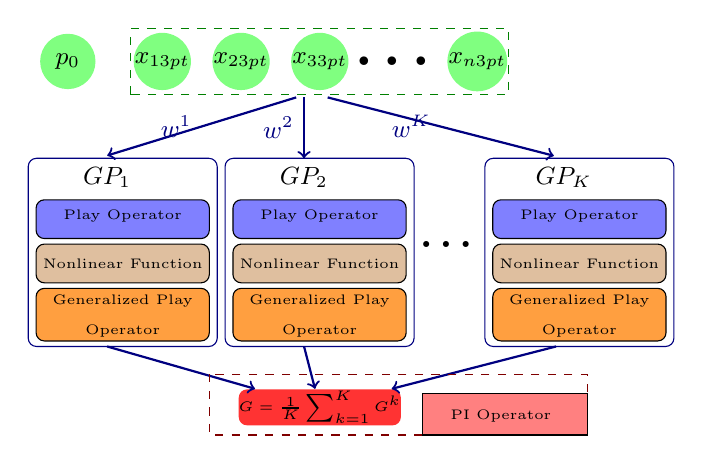
\begin{tikzpicture}[font=\small, every text node part/.style={align=center}]
                       
    \tikzstyle{neuron}=[circle,fill=black!25,minimum size=20pt,inner sep=0pt]
    \tikzstyle{input neuron}=[neuron, fill=green!50];
    \tikzstyle{hidden neuron}=[neuron, fill=blue!50];
    \tikzstyle{activation neuron}=[neuron, fill=blue!50, rectangle, rounded corners=3pt, minimum size=13pt];
    \tikzstyle{play output neuron}=[neuron, fill=red!80, rectangle, rounded corners=3pt, minimum size=13pt];
    %% draw neurons
    % \draw (0.2, 0.7) node [] {Multiple Play};
    \node[input neuron] at (-0.2,0) {$p_0$};

    \foreach \x in {1,2,3} {
        \node[input neuron] (x_\x) at (\x, 0) {$x_{\scaleto{\x}{3pt}}$};
    }
    \node[input neuron] (x_n) at (5,0) {$x_{\scaleto{n}{3pt}}$};
    \path (x_3) -- (x_n) node[midway,scale=2,font=\bfseries] {\dots};
    \draw[dashed,thin,green!50!black] (0.6,-12pt) rectangle (5.4, 12pt);
    \node[] (input) at (2.8,-10pt) {}; % make anchor here
%    \node[] at (7, 0) {$X=[x_1,x_2,...,x_n]$};
    
    \begin{scope}[xshift=-20]
    \foreach \x / \idx in {0/1,2.5/2} {
        \draw[thick,solid,rounded corners=3pt,thin,blue!50!black] (\x,-35pt) rectangle (\x+2.4, -103pt);
        % \node[] (play_\idx) at (\x+1, -35pt);
        \node[] at (\x+1, -42pt) {$GP_\idx$};
        
        \draw[solid,rounded corners=3pt,thin,fill=blue!50!white] (\x+0.1,-50pt) rectangle (\x+2.3, -64pt);
        \node[]  at (\x+1.2,-56pt) {\tiny Play Operator};
        \draw[solid,rounded corners=3pt,thin,fill=brown!50!white] (\x+0.1,-66pt) rectangle (\x+2.3, -80pt);
        \node[]  at (\x+1.2,-73pt) {\tiny Nonlinear Function};
        \draw[solid,rounded corners=3pt,thin,fill=orange!75!white] (\x+0.1,-82pt) rectangle (\x+2.3, -101pt);
        \node[]  at (\x+1.2,-92pt) {\tiny Generalized Play \\ \tiny Operator};
    }
    
    \draw[thick,solid,rounded corners=3pt,thin,blue!50!black] (5.8,-35pt) rectangle (8.2, -103pt);
    \node[] (play_k) at (6.8, -35pt) {};
    \node[] at (6.8, -42pt) {$GP_K$};
    \draw[solid,rounded corners=3pt,thin,fill=blue!50!white] (5.9,-50pt) rectangle (8.1, -64pt);
    \node[]  at (7.0,-56pt) {\tiny Play Operator};
    \draw[solid,rounded corners=3pt,thin,fill=brown!50!white] (5.9,-66pt) rectangle (8.1, -80pt);
    \node[]  at (7.0,-73pt) {\tiny Nonlinear Function};
    \draw[solid,rounded corners=3pt,thin,fill=orange!75!white] (5.9,-82pt) rectangle (8.1, -101pt);
    \node[]  at (7.0,-92pt) {\tiny Generalized Play \\ \tiny Operator};
    \end{scope}

    \path (4.5,-66pt) -- (4.8, -66pt) node[midway,scale=1.4,font=\bfseries] {\dots};

    \draw [->,color=blue!50!black,thick] (2.7,-13pt) to node [left,color=blue!50!black] {$w^1$} (0.3,-34pt);
    \draw [->,color=blue!50!black,thick] (2.8,-13pt) to node [left,color=blue!50!black] {$w^2$} (2.8,-35pt);
    \draw [->,color=blue!50!black,thick] (3.1,-13pt) to node [left,color=blue!50!black] {$w^K$} (play_k);
    
    \node[play output neuron] (output) at (3, -125pt) {\tiny $G=\frac{1}{K}\sum_{k=1}^{K}G^{k}$};
    
    \draw [->,color=blue!50!black,thick] (0.3,-103pt) to node [left,color=blue!50!black] {} (output);
    \draw [->,color=blue!50!black,thick] (2.8,-103pt) to node [left,color=blue!50!black] {} (output);
    \draw [->,color=blue!50!black,thick] (6.,-103pt) to node [left,color=blue!50!black] {} (output);
    % output dashed rect
     \draw[dashed,thin,red!50!black] (1.6,-113pt) rectangle (6.4, -135pt);
     \draw[thin,fill=red!50!white] (4.3,-120pt) rectangle (6.4, -135pt);
    \node[]  at (5.3,-128pt) {\tiny PI Operator};
    
\end{tikzpicture}
\end{document}

